%%%%%%%%%%%%%%%%%%%%%%%%%%%%%%%%%%%%
% template.tex
%
% Template for the KTHEEposter class.
%
% Original version: Mats Bengtsson, 28/5 2002
% Updated:
%   Mats Bengtsson April 2011 - July 2012
%   Manuel Olguín October 2018
%%%%%%%%%%%%%%%%%%%%%%%%%%%%%%%%%%%%

\PassOptionsToPackage{showframe}{geometry}
\documentclass[portrait, a1]{KTHEEposter}
\usepackage{lipsum}
\usepackage{listings}
\usepackage{enumitem}
\usepackage{caption}
\usepackage{subcaption}
\captionsetup{font=normalsize,labelfont={bf,sf}}
\captionsetup[sub]{font={small}, textfont={normalfont}, labelfont={bf,sf}}
\usepackage{indentfirst}
\lstset{basicstyle=\ttfamily, frame=single}
\usepackage{pgfplots}
\pgfplotsset{compat=1.14}
\usepackage[export]{adjustbox}
\usepackage{tikz}
\usetikzlibrary{shapes,arrows.meta,positioning,automata}
\usepackage{sourcecodepro}

\kthlogo{kth_eng_cmyk}
\extralogo{img/cmu_csd_logo}
\kthcolor{KTHblue}

\begin{document}
    
    \title{\LARGE\bfseries Scaling on the Edge:\\A Benchmarking Suite For Human-in-the-Loop Applications}
    
    \author{\Large M. Olguín, J. Wang, M. Satyanarayanan, J. Gross}
    \maketitle
    
    \begin{pcolumns}[3]
        \begin{pcolumn}[2]
            \begin{pframe}[.68]
                \section{Abstract}
                Benchmarking human-in-the-loop application is complex given their nature, which heavily depends on the actions taken by the \emph{human} user.
                This limits reproducibility as well as feasibility of performance evaluations.
                We propose a methodology and present a benchmarking suite we call EdgeDroid  that can address these challenges.
                Our core idea rests on recording traces of these applications which are played out in a controlled fashion based on an underlying model of human behavior.
                The traces are then exposed to the original backend compute process of the respective human-in-the-loop application, generating realistic feedback.
                This allows for an automated system which greatly simplifies benchmarking large scale scenarios.
            \end{pframe}
            \begin{pframe}[1.32]
                \section{Design \& Implementation}
                \begin{center}
                    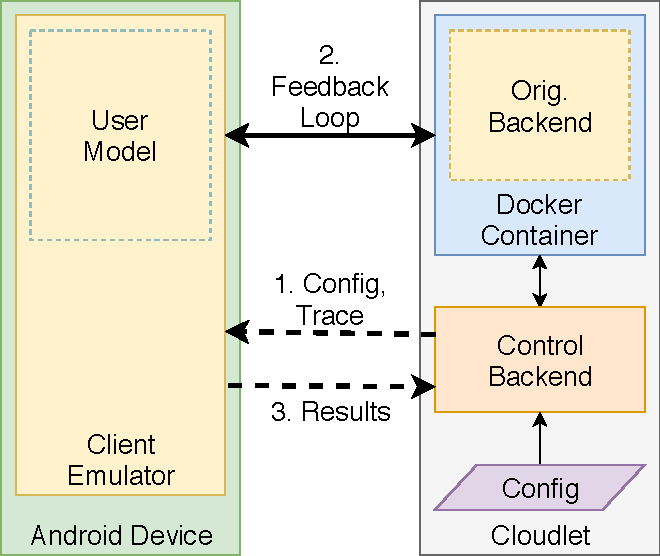
\includegraphics[width=\linewidth]{img/TraceReplay_GenArch}
                    \captionof{figure}{EdgeDroid Architecture}
                \end{center}
                
                The architecture of our benchmarking suite consists of two main components:
                \begin{itemize}
                    \item The \emph{control backend}, which controls the experiments and collects measurements from the application and the client emulators.
                    \item The \emph{client emulators}, which play out a prerecorded sensory input trace over the network in a controlled fashion.
                \end{itemize}
                
            \end{pframe}
        \end{pcolumn}%
        \begin{pcolumn}[3]
            \begin{pframe}[.9]
                \begin{center}
                    \adjustbox{scale=0.7}{
    \ttfamily\centering%\fbox{%
    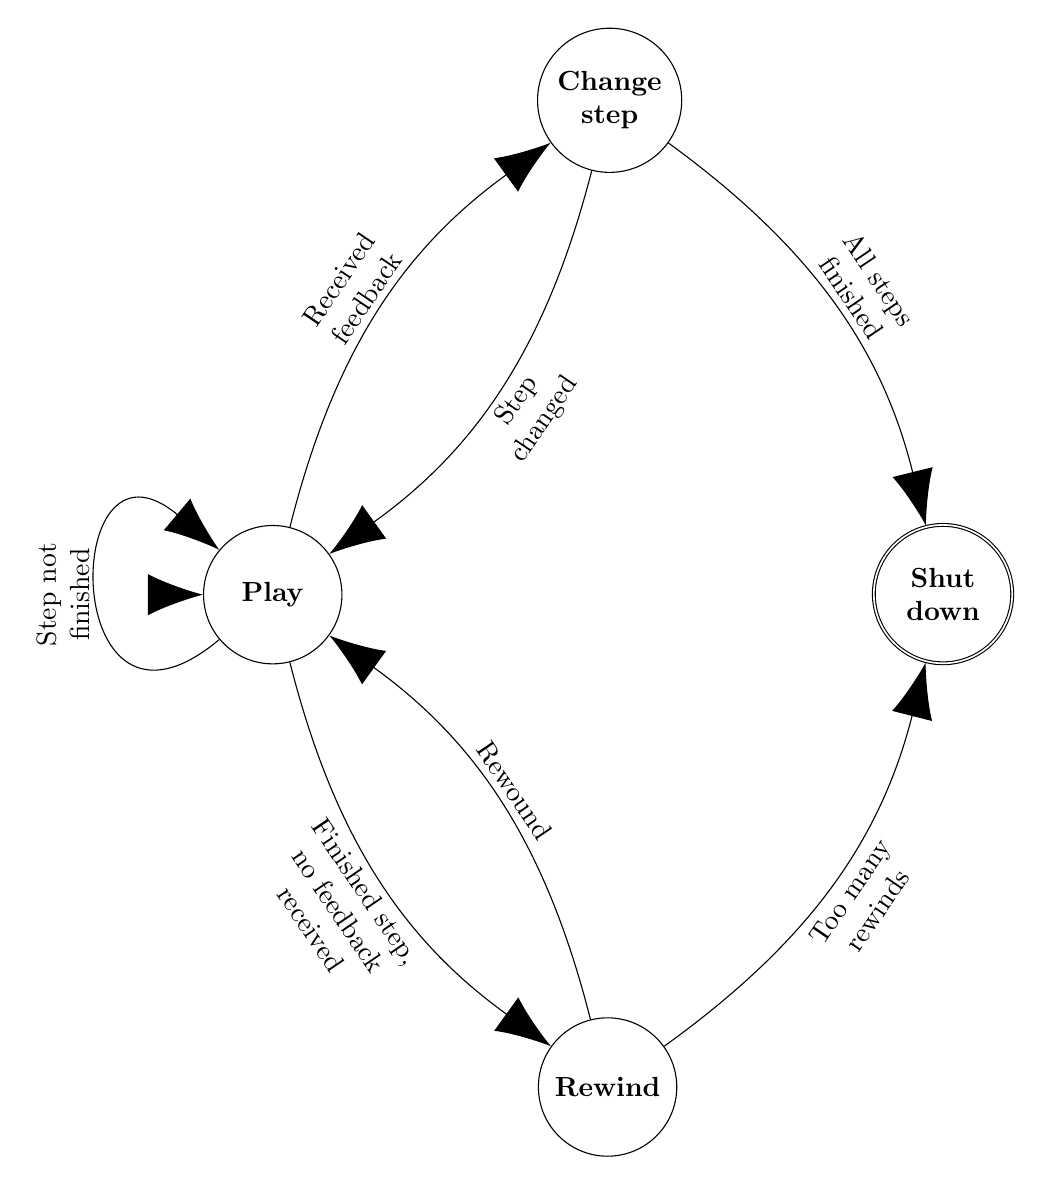
\begin{tikzpicture}[align=center,
        node distance=5cm and 3cm,
        every initial by arrow/.style={-{Latex[length=7mm]}}]
        % Place nodes              
        \node [initial, state, minimum size=5em, initial text=] (play) {\textbf{Play}};
        \node [state, above right=of play, minimum size=5em] (change) {\textbf{Change}\\\textbf{step}};
        \node [state, below right=of play, minimum size=5em] (rewind) {\textbf{Rewind}};
        \node [state, accepting, above right=of rewind, minimum size=5em] (shutdown) {\textbf{Shut}\\\textbf{down}};

        % Draw edges
        \path[draw, -{Latex[length=7mm]}, sloped, anchor=center]
        (play) edge [bend right=20] node[below] {Finished step,\\no feedback\\received} (rewind)
        edge [bend left=20] node[above] {Received\\feedback} (change)
        edge [in=140, out=220,looseness=6] node[above] {Step not\\finished} (play)

        (change) edge [bend left=20] node[below] {Step\\changed} (play)
        edge [bend left=20] node[above] {All steps\\finished} (shutdown)

        (rewind) edge [bend right=20] node[above] {Rewound} (play)
        edge [bend right=20] node[below] {Too many\\rewinds} (shutdown);

    \end{tikzpicture}
}%}
                    \captionof{figure}{Simple user model used for the initial iteration of the suite.}
                \end{center}
            \end{pframe}            
        \end{pcolumn}%
        \begin{pcolumn}[2]
            \begin{pframe}
                \section{Some Example Results}
                \begin{center}
                    
\includegraphics[width=\linewidth]{plots/comparison/box_legend.pdf}
                    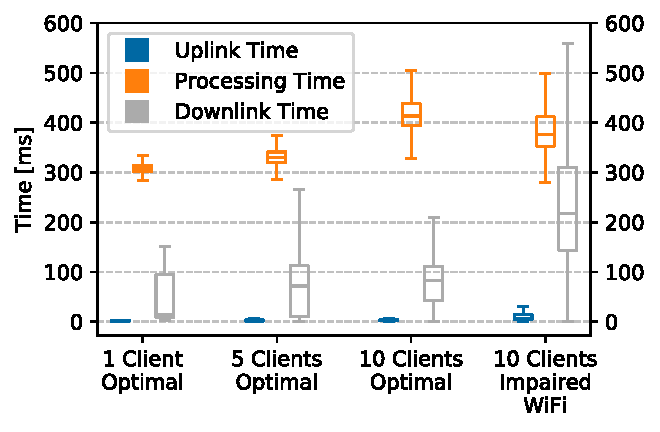
\includegraphics[width=\linewidth]{plots/comparison/box_feedback.pdf}
                    \captionof{subfigure}{Inputs that triggered feedback.}
                    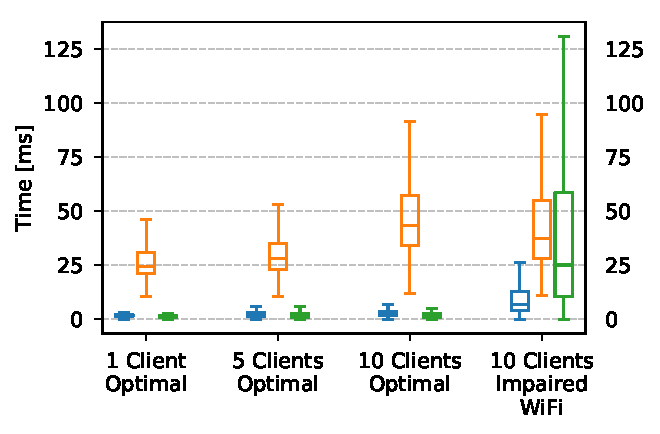
\includegraphics[width=\linewidth]{plots/comparison/box_nofeedback.pdf}
                    \captionof{subfigure}{Inputs that did not trigger feedback.}
                    \captionof{figure}{Comparison of latencies for a series of scenarios, differentiated by feedback/lack of feedback.}
                \end{center}
            \end{pframe}
            \begin{pframe**}
            \end{pframe**}
        \end{pcolumn}
    \end{pcolumns}
    
\end{document}